% ConformWeb main-body draft.
% Assumes the Overleaf project root contains figures/ and tables/ directories.
% Suggested packages: graphicx, booktabs, amsmath, amssymb, natbib.

\begin{abstract}
LLMs increasingly generate runnable web applications rather than isolated code
fragments. These applications can look complete under short demonstrations:
pages render, controls appear, forms submit, and familiar workflows begin. Yet
interactive correctness is not a property of a single screen or a local action.
It depends on whether behavior remains coherent as state, views, routes,
permissions, services, uploads, and persistence interact over time. We introduce
ConformWeb, a contract-grounded evaluation protocol for generated web
applications. A public behavioral contract serves three roles at once: it is the
generation input, the admissibility boundary for hidden scenarios, and the
source from which browser checks are compiled. Private scenarios can hide
workflow compositions, but every action, observation, and relation must compile
against the public contract, preventing hidden tests from becoming hidden
product requirements. A deterministic browser evaluator executes the compiled
scenarios, records public state and rendered evidence, and applies rule-based
checks without using an LLM judge. We instantiate the protocol in a validated
scenario collection containing 294 public scenarios and 485 private scenarios
across six application families and four complexity tiers. Across 2,160
planned blind generations, counting missing executions as failures, only 244
fully pass all private scenarios (11.3\%), while scenario-level conformance
reaches 36.3\% and step-level progress reaches 49.1\%. The gap shows that
generated apps often realize plausible surfaces and workflow prefixes, yet
fail to preserve behavioral invariants under unseen interaction compositions.
\end{abstract}

\section{Introduction}
\label{sec:introduction}

Large language models and coding agents increasingly generate runnable web
applications rather than isolated functions, scripts, or static pages
\citep{lu2025webgenbench,zhu2025frontendbench,11334714}. These applications can
look ready under a short demonstration. Pages render, controls are visible,
forms accept input, and common workflows begin as expected. But correctness for
an interactive application is not established by a single screen, a local unit
test, or a disclosed example path. A submitted form must be reflected in later
summary views. A role change must alter which actions are allowed. A file
upload must update both internal records and rendered tables. A reload must
preserve data that the interface has already claimed to save. Generated
applications often fail at exactly these boundaries while retaining a plausible
surface.

This exposes a shift in the unit of evaluation. Existing evaluations provide
important signals for code correctness
\citep{jimenez2024swebench,jain2024livecodebench,zhuo2024bigcodebench},
front-end and web generation
\citep{si2024design2code,lu2025webgenbench,zhu2025frontendbench,11334714}, and
agent task completion in existing environments
\citep{zhou2024webarena,koh2024visualwebarena,drouin2024workarena,xie2024osworld}.
In these settings, at least one side of the interaction boundary is usually
fixed before evaluation begins: the callable interface, unit-test harness,
target page, reference visual design, or environment in which an agent acts.
Generated web applications shift this boundary. The generated artifact is not
only code behind an interface; it becomes the interactive environment that
future actions must operate. The system under test must produce the controls
that actions target, the routes through which workflows proceed, the state that
later steps rely on, and the rendered evidence by which behavior is checked.
Evaluation therefore cannot assume a stable environment around the generated
code; it must evaluate whether the generated artifact has constructed such an
environment correctly.

This creates a dilemma for hidden evaluation. If tests are fully disclosed,
models can overfit short demonstrations or satisfy narrow examples without
preserving the underlying behavior. If tests are hidden without an explicit
boundary, failures may reflect undisclosed requirements rather than incorrect
implementations. Generated web applications therefore require an evaluation
discipline in which the \emph{workflow} is hidden but the \emph{behavioral
scope} is public. A private scenario should be able to choose concrete values,
order actions, and compose obligations in new ways, but every action,
observation, and check must be grounded in behavior that was declared before
generation.

We introduce ConformWeb, a contract-grounded protocol for behavioral
conformance evaluation of generated web applications. Its central object is a
public behavioral contract that plays three roles simultaneously. It is the
input from which the model generates an app. It is the admissibility boundary
that decides whether a private scenario is fair. It is also the source from
which browser actions and rule-based assertions are compiled. Evaluation is
therefore hidden in interaction sequence but public in behavioral scope. A
generated application is judged as an implementation of declared behavior, not
by visual similarity to an undisclosed target and not by matching an
undisclosed reference implementation. The contribution is not simply a new set
of tasks; it is a way to turn generated-application evaluation into admissible
hidden interaction testing.

We instantiate this protocol in a validated scenario collection. The collection
contains 294 public scenarios and 485 private scenarios, organized as a
controlled factorial instantiation rather than a flat task list. Its six
families vary the form of behavioral coupling: booking and travel state,
grocery fulfillment, clinical operations, registrar records, campaign release,
and home-service dispatch. Its four tiers increase workflow pressure from
short consumer flows to operational views, policy constraints, uploads,
deterministic services, persistence, browser history, and release-stage
synchronization. Reference implementations are used as executable witnesses
that private scenarios are attainable from the public contract, not as hidden
targets for generated applications to imitate.

Applying ConformWeb to 2,160 planned blind generations, we find that strict
behavioral conformance remains rare. Counting missing executions as failures,
244 runs pass every private scenario, for an 11.3\% full-pass rate.
Scenario-level conformance reaches 36.3\%, while step-level progress reaches
49.1\%. This gap is the central empirical signal. Generated applications often
expose requested controls and advance through substantial workflow prefixes,
yet lose consistency when later actions must honor earlier state, permissions,
rendered evidence, or persistence. ConformWeb reveals failures that screenshots,
static code inspection, short manual checks, and tests disclosed at generation
time are unlikely to expose.

Our contributions are:
\begin{itemize}
    \item We formulate generated web-application evaluation as behavioral
    conformance under interaction: correctness requires declared behavior to
    remain coherent across unseen workflow compositions, not only disclosed
    examples, local actions, or visual surfaces.

    \item We introduce ConformWeb, a contract-grounded protocol in which the
    same public contract guides generation, bounds hidden evaluation, and
    compiles into deterministic browser checks.

    \item We use ConformWeb to analyze current LLM-generated web applications
    across 2,160 planned blind generations, showing that full behavioral
    conformance remains rare despite substantial partial workflow progress and
    tracing failures to contract-facing breakdowns in state, actionability,
    routing, persistence, and rendered evidence.
\end{itemize}

\section{Related Work}
\label{sec:related}

ConformWeb relates to web-agent evaluation, code and interface generation, and
specification-based testing. The distinction is the location of the evaluation
boundary. ConformWeb targets the case where the generated artifact is the
interactive application that future browser actions will use.

\paragraph{Agents in existing interactive environments.}
Web, GUI, and computer-use benchmarks evaluate agents that act in environments
supplied by the benchmark
\citep{zhou2024webarena,koh2024visualwebarena,drouin2024workarena,xie2024osworld}.
These benchmarks test perception, navigation, tool use, and task completion in
existing worlds. Pages already exist, widgets have intended meanings, and state
transitions are implemented by the environment. ConformWeb studies the inverse
case. The generated application is the world in which evaluation occurs. The
question is not whether an agent can operate a reliable interface, but whether
an LLM-generated interface and its underlying behavior are reliable enough to
support valid future interactions.

\paragraph{Code, front-end, and web generation.}
Execution-based code benchmarks established that generated programs should be
judged by behavior rather than textual similarity
\citep{jimenez2024swebench,jain2024livecodebench,zhuo2024bigcodebench}.
Front-end and web-generation benchmarks extend evaluation to rendered pages,
components, and user-facing artifacts
\citep{si2024design2code,lu2025webgenbench,zhu2025frontendbench,11334714}.
These settings provide valuable signals, but they often fix a callable
interface, target design, component boundary, or local task. Generated web apps
introduce a different failure mode. A page can render convincingly, accept
inputs, and satisfy a local check, yet fail when later views, permissions,
routes, service responses, persistence, or derived evidence must remain
consistent with earlier actions. ConformWeb evaluates browser-observable
behavior over stateful workflows rather than only unit-level functionality,
visual similarity, or isolated interface behavior.

\paragraph{Specification and conformance testing.}
Specification-based testing, model-based testing, property-based testing, and
conformance testing provide the broader principle that systems should be judged
against declared behavior. GUI and web testing further show that many faults
appear only through event sequences, navigation paths, and interaction
histories. ConformWeb adopts this principle in a generated-artifact setting
where the public specification has three simultaneous roles. It guides
application generation, defines the admissible scope of hidden scenarios, and
supplies the basis for executable browser checks. This differs from applying a
test specification to an already-given system. The protocol must also ensure
that private workflows are hidden without becoming hidden product
requirements. Reference implementations therefore serve as witnesses that the
public contract is sufficient, not as secret targets that generated apps must
imitate.

\section{ConformWeb Protocol}
\label{sec:protocol}

ConformWeb is a protocol for asking whether a generated web application
implements declared behavior under interaction. Each instance contains a
product premise, a public behavioral contract, public scenarios, and private
scenarios. The premise fixes the application setting. The contract declares the
behavioral scope. Public scenarios provide representative disclosed workflows.
Private scenarios provide held-out workflow compositions. Crucially, private
scenarios are valid only when every action, evidence channel, and check is
grounded in the public contract.

The protocol separates three questions. \emph{Surface realization} asks whether
the generated app exposes the declared controls and evidence surfaces.
\emph{Public-scenario conformance} asks whether it satisfies disclosed
workflows. \emph{Private-scenario conformance} asks whether the same declared
obligations hold under unseen compositions. This separation distinguishes apps
that omit required surfaces, apps that fail disclosed workflows, and apps that
appear plausible until stateful obligations compose.

The protocol is built around three invariants. First, \emph{public scope}: any
behavior evaluated in private must be declared before generation. Second,
\emph{hidden composition}: private scenarios may recombine declared actions,
values, roles, routes, and checks in orders not shown to the model. Third,
\emph{deterministic audit}: the evaluator executes browser plans and checks
structured observations without an LLM judge. These invariants are what turn a
collection of browser tests into a conformance protocol for generated
applications.

\subsection{Protocol Object}
\label{sec:protocol-object}

Classical conformance testing typically assumes an implementation whose
interface and operating environment already exist. ConformWeb changes this
object of evaluation. The generator must construct the environment that the
hidden test will later operate. Formally, an evaluation instance contains a
product premise \(x\), public contract \(C\), public scenarios \(P_C\), and
private scenarios \(T_C\). A model produces
\begin{equation}
G = M(x,C,P_C),
\end{equation}
and the evaluator scores \(G\) only on private scenarios satisfying
\begin{equation}
\forall \tau\in T_C,\quad \tau \preceq C .
\end{equation}
The executable evaluator is itself derived from the public boundary,
\begin{equation}
E_C = \mathrm{compile}(C,T_C).
\end{equation}
The same contract therefore binds both sides of the evaluation: it constrains
what the model was asked to build, and it constrains what hidden scenarios are
allowed to test.

This is the qualitative difference from a collection of hand-written end-to-end
tests. In ordinary end-to-end testing, a hidden test can be fair because the
interface is already fixed by an existing application or API. In generated web
applications, the interface is part of the generated output. Without an
admissibility relation \(\tau\preceq C\), a hidden browser test can silently
become a hidden product requirement. ConformWeb makes that boundary explicit:
private scenarios may be unseen, but their vocabulary and relations must be
public.

\subsection{Public Contracts}
\label{sec:contracts}

The public contract is the boundary that makes hidden evaluation fair. It
declares what may be done, what may be observed, and what may be checked. We
represent a contract as
\begin{equation}
C=(\mathcal{A}_C,\mathcal{O}_C,\mathcal{R}_C),
\end{equation}
where \(\mathcal{A}_C\) is the set of admissible browser actions,
\(\mathcal{O}_C\) is the observation surface, and \(\mathcal{R}_C\) is the set
of behavioral relations that can be checked over observations. Actions include
control operations, input updates, uploads, role changes, navigation, browser
history traversal, and reloads. Observations include public application state,
browser metadata, deterministic service calls, and rendered projections such
as table rows. Relations include state transitions, validation behavior,
authorization effects, route and persistence obligations, service outcomes, and
rendered-projection consistency.

The contract is not merely a prompt format. It is also the static namespace for
private evaluation and the semantic input to the browser evaluator. This is
what prevents two common failure modes. Hidden scenarios cannot ask for
behavior outside the contract, and generated apps cannot receive credit for
plausible screens whose observable behavior is absent from the declared
surface. The contract also does not prescribe a source-code architecture. A
generated application may use any internal state representation or framework.
It is evaluated only through the declared interaction and observation surfaces.

In our instantiation, contracts are machine-readable objects rather than free
form natural-language instructions. They declare component selectors, public
state paths and types, routes, roles, service fixtures, upload schemas,
rendered-table schemas, persistence obligations, and relation types. This
structure is what lets the same contract be used by the generator, the
admissibility checker, and the evaluator. Natural language supplies the product
premise, but the conformance boundary is the structured contract.

\paragraph{Example.}
Consider a grocery-style contract that declares an \textsc{AddItem} action, a
public state path for the cart count, a rendered cart table, and a relation
stating that adding an item increases the count and projects the item into the
table. A private scenario may choose a new item value, add it before checkout,
reload the page, and then check that both the state count and rendered table
remain consistent. This scenario is hidden in composition and concrete values,
but it is public in behavioral scope. By contrast, a private check for an
undeclared loyalty discount or an undeclared inventory policy would be rejected
before scoring because it cannot be derived from \(C\).

\subsection{Admissible Private Scenarios}
\label{sec:admissibility}

A private scenario \(\tau\) is admissible under contract \(C\), written
\(\tau \preceq C\), only if all of its references resolve through the public
contract. Each action must instantiate an element of \(\mathcal{A}_C\), each
observation reference must be drawn from \(\mathcal{O}_C\), and each check must
instantiate a relation in \(\mathcal{R}_C\). Arguments to these actions and
checks may use only declared selectors, roles, routes, service fixtures, upload
schemas, tables, state paths, and evidence channels.

This admissibility condition is the core fairness constraint. A private
scenario may select new values, order declared actions, and compose declared
obligations in unseen ways. It may not introduce new product requirements. If a
scenario cannot be compiled from the public contract, its failure is a
construction error in the evaluation instance rather than a
generated-application failure. Admissibility therefore moves fairness from an
informal after-the-fact argument into a checkable property of the scenario
itself.

This also distinguishes public examples from public scope. Public scenarios
are disclosed workflows; they need not enumerate every behavior that can be
tested. A private scenario may use a declared action, state path, route, or
rendered table that does not appear in a public scenario, but it remains
admissible only if that reference is declared in the public contract. The
model's generalization target is therefore recombination within a declared
behavioral namespace, not guessing an undisclosed product feature.

\subsection{Trace Semantics}
\label{sec:trace-semantics}

For a generated application \(G\) and an admissible private scenario
\(\tau=((a_i,Q_i))_{i=1}^{n}\), execution produces a browser trace
\begin{equation}
o_0,a_1,o_1,\ldots,a_n,o_n ,
\end{equation}
where \(a_i\in\mathcal{A}_C\) and \(Q_i\) is the finite set of checks evaluated
after action \(a_i\). The initial observation \(o_0\) is recorded before the
first action, and \(o_i\) is recorded after action \(a_i\). A step passes when
the declared action is executable and all corresponding checks hold:
\begin{equation}
\mathrm{pass}_i(G,\tau)=
\mathrm{exec}_G(a_i)
\land
\bigwedge_{q\in Q_i} q(o_{i-1},o_i).
\end{equation}
The application satisfies the scenario when every step passes:
\begin{equation}
G\models_C \tau
\iff
\forall i\in\{1,\ldots,n\},\ \mathrm{pass}_i(G,\tau).
\end{equation}

The term \(\mathrm{exec}_G(a_i)\) makes actionability part of conformance. A
named element is insufficient if it is hidden, disabled, covered, absent in the
required workflow state, or otherwise unavailable to the browser action.
Asynchronous behavior is handled through contract-declared waits or completion
conditions inserted into the compiled plan, so timing tolerance remains part of
the evaluation specification rather than a private evaluator heuristic.

\subsection{Compilation and Observation}
\label{sec:compilation}

ConformWeb compiles admissible scenarios into browser plans. This compilation
step is the mechanism that connects the public contract to executable
evaluation: the evaluator is not a separate hand-written oracle, but a
deterministic lowering of declared actions and relations. Each semantic step is
lowered into the pattern
\begin{equation}
\textsc{observe}_{pre}
\rightarrow
\textsc{act}
\rightarrow
\textsc{observe}_{post}
\rightarrow
\textsc{check}.
\end{equation}
The compiler rejects undeclared actions, pages, actors, events, rendered
tables, state paths, modes, and check operators before scoring. The browser
runner then executes the plan in a fresh browser context, interacts through
declared selectors and browser operations, records before/after screenshots,
and evaluates rule-based assertions over the captured evidence.

An observation has structured views
\begin{equation}
o_i=(s_i,b_i,v_i,q_i),
\end{equation}
where \(s_i\) is public application state, \(b_i\) is browser metadata,
\(v_i\) is rendered UI evidence declared by the contract, and \(q_i\) records
deterministic service interactions. Screenshots are stored for audit, but they
are not used as aesthetic judgments. No language model is used as a judge.

The evaluator is strict only where the contract is explicit: selectors, state
paths, routes, and rendered-table schemas are public obligations of the
generated application. This differs from open-ended visual grading, where
failures may depend on ambiguous human or model judgments. When a browser
action cannot execute or a relation cannot be evaluated, the failure is
reported through the same contract-facing evidence surface used for successful
checks.

This design does not claim to measure every dimension of web-app quality. It
does not score aesthetics, maintainability, or behavior outside the public
contract. Its goal is narrower and auditable: if an app exposes a declared
control, state path, route, service, or rendered projection, then hidden
scenarios may test whether those declared obligations remain coherent under
interaction. Potential false negatives are therefore localized to explicit
contract obligations, and validation artifacts make them inspectable.
Conversely, a passing result is not a proof of complete application quality; it
is conformance to the declared behavioral contract.

\subsection{Scores and Failure Evidence}
\label{sec:scores}

Let \(T_C\) be the private scoring scenarios for contract \(C\). The primary
score is strict scenario-level conformance:
\begin{equation}
S_{\mathrm{scen}}(G)=
\frac{\sum_{\tau\in T_C} w_\tau \mathbf{1}[G\models_C\tau]}
     {\sum_{\tau\in T_C} w_\tau}.
\end{equation}
A scenario receives credit only when all compiled checks pass. We also report
step-level progress:
\begin{equation}
S_{\mathrm{step}}(G)=
\frac{\sum_{\tau\in T_C} w_\tau p_\tau(G)}
     {\sum_{\tau\in T_C} w_\tau}.
\end{equation}
For \(\tau\) with \(n_\tau\) steps, \(p_\tau(G)=\ell_\tau(G)/n_\tau\), where
\(\ell_\tau(G)\) is the longest prefix in which every step passes. Thus
\(p_\tau(G)=1\) exactly when \(G\models_C\tau\), while lower values indicate
how far the application progressed before the first failed action or check.

For each failed scenario, the evaluator records the first failing step, failed
assertion or browser error, expected and observed values when available, and
before/after screenshots. These artifacts make failures auditable at the level
of the contract: missing interaction surface, invalid observation surface,
unavailable action, wrong state transition, route or persistence drift, and
rendered-projection mismatch.

\section{Protocol Instantiation}
\label{sec:instantiation}

We instantiate ConformWeb in 24 web-application instances formed by crossing
six product families with four complexity tiers. The purpose of this collection
is to exercise the protocol under controlled variations in behavioral coupling.
The design is factorial: the family axis changes the product structure, while
the tier axis changes the interaction pressures applied to that structure. Each
instance tests whether the same public-contract boundary remains meaningful
when workflows introduce different combinations of state, views, routes, roles,
services, uploads, persistence, and rendered evidence.

\subsection{Families}
\label{sec:families}

The six families are chosen for different interaction structures rather than
for domain labels alone. Travel workflows stress booking state, itineraries,
checkout, and concierge updates. Grocery workflows stress cart state,
fulfillment, inventory-like constraints, support tickets, cold-chain review,
and dispatch readiness. Clinical command workflows stress regulated operational
state, escalation, handoff packets, authorization, and seal or reseal gates.
Campus registrar workflows stress institutional records, enrollment decisions,
policy-constrained updates, and multi-view student state. Media campaign
workflows stress asset review, campaign approval, launch readiness, and release
coordination. Home-service workflows stress repair intake, technician dispatch,
parts readiness, quality assurance, insurance, and warranty completion.

Across these families, the shared question is whether a generated app preserves
declared behavior under interaction. The family axis is therefore a form of
protocol stress testing. It reduces the chance that results reflect one
interface convention, vocabulary, or product shape, and it gives the error
analysis multiple opportunities to observe boundary failures between state and
rendered evidence, role and permission, service response and derived state, and
persistence claim and reload behavior.

\subsection{Tiers}
\label{sec:tiers}

Each family has four tiers. Tier A, Consumer, emphasizes short user workflows
and local consistency. Tier B, Operational, adds staff or operational views,
ordered collections, derived counters, status changes, and rendered tables.
Tier C, Regulated, adds role effects, policy constraints, deterministic
services, uploads, conflict branches, and persistent records. Tier D,
Release-stage, extends workflows to final approval, release, reopen, or
synchronization steps where multiple views and public ledgers must remain
consistent after longer interaction histories.

The tier progression is not only a length increase. Later tiers add behavioral
coupling: routes must agree with browser state, rendered tables must agree with
public records, unauthorized actions must have declared effects, uploads and
services must update derived state, and final workflow actions must synchronize
several public views. This structure lets the protocol distinguish immediate
surface failures from applications that make progress before drifting.

\subsection{Reference Validation and Disclosure}
\label{sec:validation}

Each instance is admitted only after executable validation. We first write the
premise, public contract, public scenarios, and private scenarios. The compiler
checks that private scenarios are admissible under the public contract. A
reference application is then used as an executable witness that the declared
private scenarios are attainable and that the evaluator can recognize a
conforming implementation. The reference is not disclosed to experimental
generators and is not treated as a hidden visual or source-code target. Its
role is to validate the evaluation instance, not to define the desired
implementation.

This validation gives two independent checks on hidden-scenario fairness. The
static check ensures that every private reference is declared by the public
contract. The executable check ensures that the resulting private scenarios can
be satisfied by at least one implementation built for the same public behavior.
Together, these checks make the hidden evaluation boundary inspectable before
any generated application is scored.

The two checks serve different purposes. Static admissibility prevents private
scenarios from referring to behavior outside the public contract. Reference
validation checks executability of the resulting obligations. Passing the
reference does not define the target behavior; the contract does. The reference
only witnesses that the contract and private scenarios are jointly satisfiable
by an implementation.

Experimental generators receive the product premise, public contract, and
public scenarios. They do not receive private scenarios, reference code,
reference screenshots, execution traces, evaluator output, or failure feedback.
This disclosure boundary is fixed across families and tiers.

\begin{figure*}[t]
    \centering
    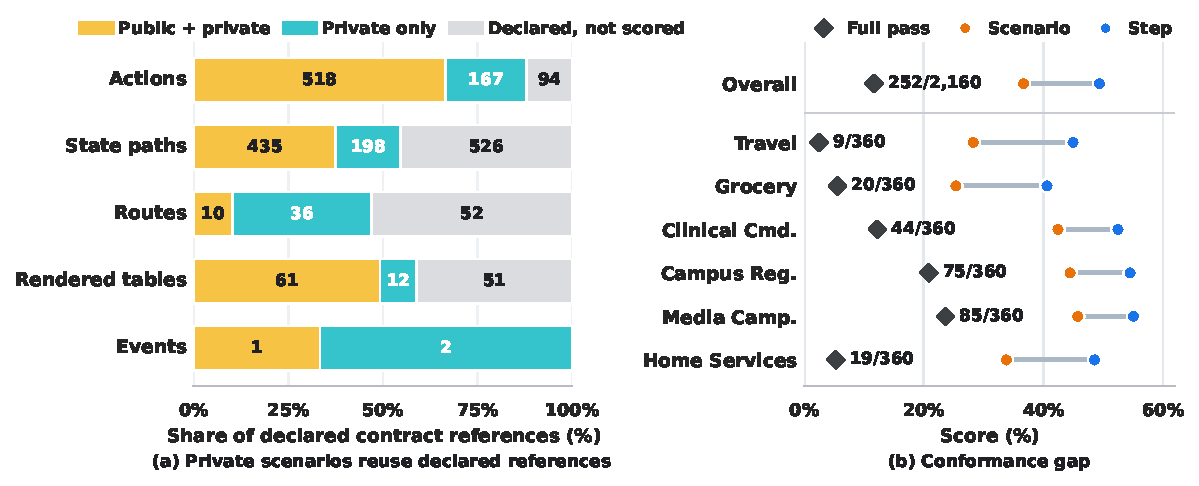
\includegraphics[width=.92\textwidth]{figures/main/figure_admissibility_conformance_gap.pdf}
    \caption{
    ConformWeb hides workflow composition while keeping behavioral scope public.
    The left panel audits whether private scenarios reuse references declared
    in the public contract; references used only in private scenarios are still
    public declarations. The right panel shows that generated apps often make
    partial progress but rarely satisfy all private scenarios end to end.
    }
    \label{fig:admissibility-gap}
\end{figure*}

Figure~\ref{fig:admissibility-gap} summarizes the two sides of the protocol.
The private-scenario audit shows that held-out checks are grounded in declared
references rather than undisclosed product requirements. The conformance plot
then shows why hiding compositions matters: generated apps often make partial
progress while failing strict end-to-end conformance.

The audit is intentionally static and semantic rather than empirical. It does
not ask whether a generated application passes. It asks whether every private
reference is legal before any generated application is evaluated. In the
current instantiation, the audited private scenarios cover 485 private
scenarios, 4,317 private steps, and 40,944 compiled checks, with no undeclared
private references. Some private scenarios use references not shown in public
scenarios, but those references are still declared in the public contract. This
is the admissibility discipline that separates hidden workflow composition
from hidden product requirements.

\section{Experiments}
\label{sec:experiments}

The experiments ask whether current LLMs can generate web applications that
preserve public behavioral contracts under private browser scenarios. They are
not intended as a definitive model leaderboard. Model variation is used to test
whether capability closes the gap between partial workflow progress and strict
behavioral conformance. Family and tier variation is used to test whether the
same protocol exposes failures as behavioral coupling changes.

\subsection{Setup}
\label{sec:setup}

We evaluate the 24 validated instances described above. Each instance follows
the same sampling plan: three capability groups, three models per group, and
ten independent generations per model, for 2,160 planned generations. The Mini
group contains GPT-5.4 nano, Claude Haiku 4.5, and Gemini 3.1 Flash Lite. The
Turbo group contains GPT-5.4 mini, Claude Sonnet 4.6, and Gemini 3.1 Flash.
The Frontier group contains GPT-5.4, Claude Opus 4.6, and Gemini 3.1 Pro
Preview.

For reproducibility, collected implementations are packaged as static browser
apps with one HTML file, one CSS file, and one JavaScript file. This packaging
constraint belongs to the experimental harness, not the protocol. ConformWeb
scores browser-observable behavior through declared selectors, state probes,
service calls, rendered evidence, and browser metadata. The protocol therefore
applies to any implementation architecture that exposes the declared
interaction and observation surfaces. We use the static packaging constraint to
hold deployment and build tooling constant across models; it is not part of the
definition of behavioral conformance.

The evaluator is a deterministic Playwright and Chromium runner. It loads each
submitted app in a fresh browser context, executes compiled private scenarios,
records public state and rendered evidence before and after each step, and
applies rule-based assertions. Missing executions are counted as failures in
planned-denominator figures. We report both accounting views: the realized
aggregate contains 2,157 executed generations, while the planned denominator is
2,160 after counting three missing executions as failures. Appendix tables
report the corresponding run accounting, prompt hashes, contract hashes,
provider-resolved identifiers, and excluded-run notes.

\subsection{Conformance Gap}
\label{sec:results-gap}

Across 2,160 planned runs, 244 pass every private scenario, yielding an 11.3\%
full-pass rate. The realized denominator gives the same rounded rate:
244/2,157. Scenario-level conformance is 36.3\%, and step-level progress is
49.1\%. The gap between these scores is the main result, not the ranking of
individual models. Generated apps often implement enough of the surface and
local logic to pass many intermediate checks, but still fail before satisfying
all private workflow obligations.

The family-level pattern in Figure~\ref{fig:admissibility-gap} shows that this
is not confined to one product shape. Travel, Grocery, Clinical Command,
Campus Registrar, Media Campaign, and Home Services all show higher
step-level progress than full-pass rate. The strict full-pass metric is
deliberately demanding: in a checkout, registration, campaign release, repair,
or clinical handoff workflow, one broken role gate, upload-derived counter,
route transition, rendered table, or final ledger update can invalidate the
end-to-end behavior.

The step-level metric is included precisely because strict conformance is
conjunctive. It prevents two distinct failures from being collapsed: an app
that never exposes the required surface and an app that follows most of a
workflow before violating a later invariant. We therefore interpret full pass
as end-to-end conformance, scenario score as strict held-out success over
private workflows, and step progress as a diagnostic prefix measure rather
than a substitute for correctness.

\subsection{Capability and Difficulty}
\label{sec:capability-difficulty}

Capability improves progress more than completion. Mini models fully pass
5/720 planned runs, Turbo models pass 65/720, and Frontier models pass 174/720.
Scenario-level conformance rises from 11.1\% for Mini to 31.6\% for Turbo and
66.1\% for Frontier. Step-level progress rises from 25.0\% to 43.9\% and
78.3\%, respectively. The same ordering appears across metrics, but the
full-pass rate remains much lower than step-level progress even for Frontier
models. This pattern answers a protocol-level question: better generation can
extend the prefix of correct behavior without eliminating failures in composed
obligations.

\begin{figure*}[t]
    \centering
    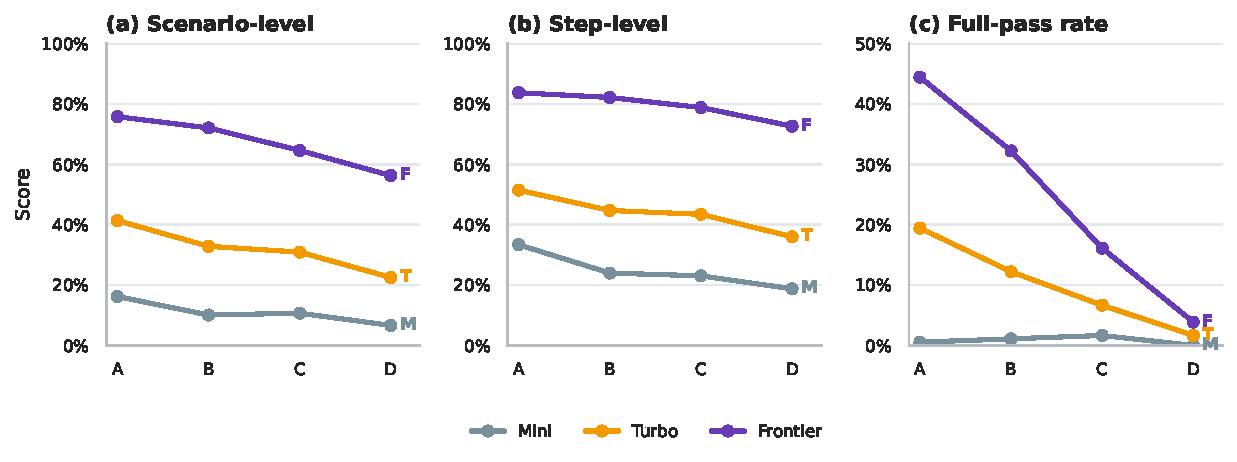
\includegraphics[width=.92\textwidth]{figures/main_or_appendix/figure_difficulty_scaling_curve.pdf}
    \caption{
    Difficulty scaling across tiers. Tier A is Consumer, Tier B is Operational,
    Tier C is Regulated, and Tier D is Release-stage. Later tiers add
    behavioral coupling through operational views, roles, services, uploads,
    rendered projections, persistence, browser history, and release
    synchronization.
    }
    \label{fig:difficulty-scaling}
\end{figure*}

Figure~\ref{fig:difficulty-scaling} shows the tiered pattern. Later tiers are
not merely larger versions of the same task. They require multiple views,
browser state, role policies, deterministic services, rendered evidence, and
final workflow ledgers to remain consistent under longer compositions. The
decline across tiers supports the interpretation that the protocol is exposing
behavioral coupling rather than only surface completion.

The tier breakdown makes this pressure visible. Full-pass counts fall from
116/540 planned runs at Tier A to 82/540 at Tier B, 38/540 at Tier C, and
8/540 at Tier D. Scenario-level conformance drops from 44.5\% at Tier A to
28.3\% at Tier D, while step-level progress drops from 56.3\% to 42.6\%.
This is the empirical role of the tier design: it distinguishes local surface
realization from the ability to preserve state, permission, route, service,
rendered-table, and persistence obligations as workflows become more coupled.

\section{Error Analysis}
\label{sec:error}

ConformWeb failures differ in both kind and timing. For each failed private
scenario, we analyze the first step after the longest passing prefix. This
gives one comparable diagnosis point per failed scenario and avoids counting
downstream violations that may follow from an earlier error.

\begin{figure*}[t]
    \centering
    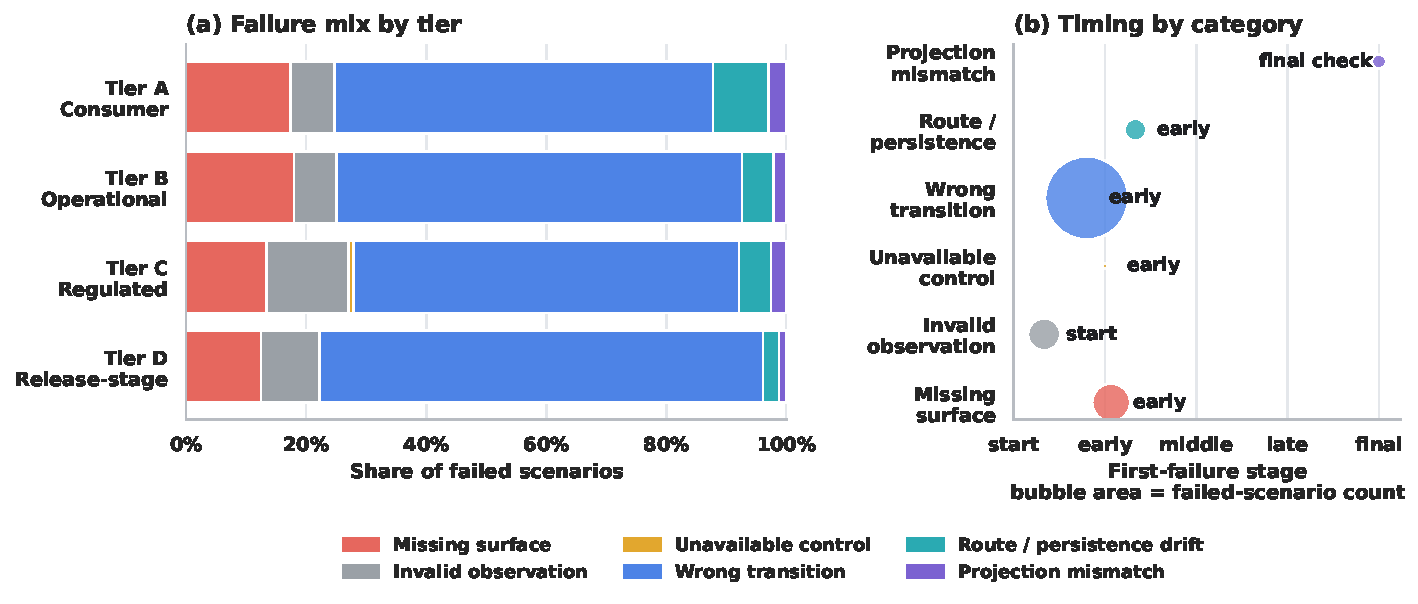
\includegraphics[width=.92\textwidth]{figures/main/figure_failure_taxonomy.pdf}
    \caption{
    First-failure patterns. The left panel shows the failure mix by complexity
    tier. The right panel shows where each category first appears, with bubble
    area indicating failed-scenario count. Later failures mainly reflect route,
    persistence, and rendered-projection drift after longer workflow prefixes.
    }
    \label{fig:failure-taxonomy}
\end{figure*}

Figure~\ref{fig:failure-taxonomy} groups first failures by the contract surface
that breaks first: missing interaction surface, invalid observation surface,
unavailable action, wrong state transition, route or persistence drift, and
rendered-projection mismatch. These labels are contract-facing rather than
source-code-facing. They describe how an executable application violates the
public behavioral contract when used through a browser.

The dominant pattern is not blank pages or obvious crashes. Many generated apps
are runnable systems that preserve enough interface structure to make progress,
but lose conformance when behavior must remain consistent across surfaces.
Actions execute without the required state transition. State changes without
the rendered projection. Role changes fail to produce the corresponding
permission effect. Reloads preserve a plausible screen while losing public
state. Final workflow actions update one ledger but not another. These are
boundary failures between what the interface appears to support and what later
observations reveal.

Capability scaling changes the failure mix more than it removes failures.
Among private scenario failures in the available raw traces, Mini models show
more early surface and observation problems: missing interaction surface and
invalid observation surface account for 23.4\% and 12.1\% of Mini failures.
For Frontier models, these categories fall to 9.5\% and 2.8\%, while wrong
state transition accounts for 82.5\% of failures. In other words, stronger
models more often build an operable surface, but remaining failures concentrate
in behavioral semantics: the action runs, yet the post-action public state,
rendered evidence, route, or persistence obligation is wrong.

Failure timing shows the same shift. Invalid observation failures are usually
immediate, with median progress 0.0 before failure. Route or persistence drift
appears later, with median progress 0.25. Rendered-projection mismatches are
rarer but much later, with median progress 0.875 in the available raw traces.
These late mismatches are especially important for generated web apps: they
can be invisible in a short demonstration because the app has already completed
many actions before the rendered evidence diverges from the declared state.

This error profile explains why the protocol reports both scenario-level
conformance and step-level progress. A low score with little progress indicates
an immediate surface or wiring failure. A low scenario-level score with high
step-level progress indicates a more subtle failure: the app approximates the
workflow, but loses an invariant under composition. ConformWeb is designed to
make that distinction observable.

\section{Conclusion}
\label{sec:conclusion}

ConformWeb evaluates LLM-generated web applications as behavior-preserving
systems under interaction. A public contract declares the actions,
observations, and relations that may be tested; private scenarios hide workflow
composition while remaining admissible under that contract; a deterministic
browser evaluator executes those scenarios and records auditable evidence. In
our current instantiation, only 244 of 2,160 planned blind generations pass
all private scenarios, even though scenario-level conformance and step-level
progress are substantially higher. The result is evidence about the evaluation
boundary, not primarily a scale claim about a collection of tasks: plausible
generated interfaces often preserve workflow prefixes without preserving the
behavioral invariants that make an interactive application correct.
Contract-grounded evaluation makes that failure mode explicit, executable, and
auditable.
